%input "worldcup.bib"

\documentclass[a4paper,11pt]{article}
%\documentclass[a4paper]{sig-alternate}
\sloppy % makes TeX less fussy about line breaking

\oddsidemargin  0.0cm
\evensidemargin 0.0cm
\textheight     22cm
\textwidth      16cm

%double space
\renewcommand{\baselinestretch}{1.4}

%The papers should not be longer than 25-30 pages, single column, double space, 11 or 12 pt font, including figures, tables and references. If the submitted papers are extensions of existing conference publications, the authors must submit a corresponding letter, specifying clearly what is new in the journal paper and how the submitted paper distinguishes itself from the published conference paper.

% COMMENTS
% motivate why we did another experiment. Maybe in content
% Are new/old same or different, and why?
% What do these charactisation mean?

% Say when we aggregated results... and run stats test to proof they are similar. ARGHHH

% Think about impact of models, and the shape of the models

% Notes
% Bookmark is a pointer, a hotspot a segment
% You a pre-fetching chunks, so the hit rate depends on how much you are pre-fetching
% Algorithm to determine length of hotspot
% Broader overview of CDN strategies
  % Explain more CDN, put into context
  % Step back, how are these exploitable?
  % 3.10 summary. Results, Benefits, and some of the things we tried
  % Paint a picture

%TODO
    % Write changes letter
    % Change all values to 3sf (to be consistent)
    % Write conclusion
    % Replot CDFs to have 0-1 on the yaxis in increments of 0.1
    % Improve related work
    %  - check "Delving into Internet Streaming Media Delivery: A Quality and Resource Utilization Perspective"
    % Check all captions



\usepackage{subfig}

\usepackage{epsfig}
\usepackage{multirow}

%for PDF features - http://www.ce.cmu.edu/~kijoo/latex2pdf.pdf
\usepackage[pdftex,colorlinks]{hyperref} % For the bookmark/hyperlinks

% style of the figure captions
\newcommand{\capttext}{\protect\centering\em}

% for the algorithm
\usepackage{algorithm}
\usepackage{algorithmic}

% for some diagrams
\usepackage{tikz}
\usetikzlibrary{arrows,snakes,backgrounds}
% line spacing
\usepackage{setspace}

%\setlength{\pdfpagewidth}{8.5in}
%\setlength{\pdfpageheight}{11in}

\hypersetup{%
    pdftitle={Characterising and Exploiting Workloads of Highly Interactive Video-on-Demand},
    pdfauthor={Andrew Brampton, Andrew MacQuire, Michael Fry, Idris A. Rai, Nicholas J. P. Race and Laurent Mathy},
    pdfkeywords={Interactive, Video-on-Demand, Sports, Worldcup, Content Distribution},
    bookmarksnumbered,
    pdfstartview={FitV},
    linkcolor={black},%: Color for normal internal links.
    anchorcolor={black},%: Color for anchor text.
    citecolor={black},%: Color for bibliographical citations in text.
    filecolor={black},%: Color for URLs which open local files.
    menucolor={black},%: Color for Acrobat menu items.
    urlcolor={black}%: Color for linked URLs.
}

\newcommand{\todo}[1]{
    %\fcolorbox{red}{white}{
    \fbox{
        \color{red}
        \small
        \sf TODO: #1
    }
}

% todo convince Michael to become a member of Lancaster University so I don't have to do nasty hacks to make this look nice
%\author{
%    Andrew Brampton$^*$ \and
%    Andrew MacQuire$^*$ \and
%    Michael Fry$^\dagger$ \and
%    Idris A. Rai$^*$ \and
%    Nicholas J.P. Race$^*$ \and
%    Laurent Mathy$^*$
%    \end{tabular}\\\tiny~\\
%    \begin{tabular}{cc}
%    \normalsize $^*$ Lancaster University & \normalsize $\dagger$ University of Sydney \\
%    \small\{brampton,macquire,rai,race,laurent\}\\\small@comp.lancs.ac.uk & \small michael.fry@usyd.edu.au \\
%}

\author{
\begin{tabular*}{0.8\textwidth}{@{\extracolsep{\fill}} c c c}
    Andrew Brampton$^*$ & Andrew MacQuire$^*$ & Michael Fry$^\dagger$ \\
    Idris A. Rai$^*$ & Nicholas J. P. Race$^*$ & Laurent Mathy$^*$ \\
\end{tabular*}\\
\begin{tabular*}{0.8\textwidth}{@{\extracolsep{\fill}} l  r}
\parbox{0.4\textwidth}{\centering\small\singlespacing $^*$ Lancaster University\\\{brampton,macquire,rai,race,laurent\}\\@comp.lancs.ac.uk} & \parbox{0.4\textwidth}{\centering\small\singlespacing $\dagger$ University of Sydney\\michael.fry@usyd.edu.au}
\end{tabular*}
}

\date{}

\begin{document}

\title{Characterising and Exploiting Workloads of Highly Interactive Video-on-Demand}
\maketitle

\begin{abstract}
  This paper presents a detailed characterisation of user behaviour
  for a series of interactive video experiments over a 12 month
  period, in which we served popular sporting and musical content. In
  addition to generic VCR-like features, our custom-built
  Video-on-Demand application provides advanced
  interactivity features such as bookmarking. The dramatic impact of
  such functionality on how users consume content is studied and
  analysed. We discuss in detail how this dynamic user behaviour can
  be exploited by content distributors to improve user
  experience. Specifically, we study how simple dynamic bookmark placement
  and interactivity-aware content pre-fetching and replication can
  reduce the impact of highly interactive media on CDN performance.
\end{abstract}

\section{Introduction}

In recent years the Internet has increasingly been used to distribute
bandwidth-intensive, low-latency streaming media. Due to the resources
required to deliver such content, dedicated Content Distribution
Networks (CDNs) are often used to improve the experience of end-users. As such systems evolve, users expect correspondingly
improved interactive functionality, something which is increasingly
difficult to achieve with diverse content types exhibiting varied
access patterns. In order to provide a high quality of service, modern
CDNs must therefore be optimised to respond to user behaviour
regarding different content types.

In this paper, we study user behaviour for an interactive
Video-on-Demand (VoD) system that serves users with a range of
content. Broadly, we served videos in the sporting and musical genres,
with respective examples being the entire 2006 FIFA World Cup and 2007
Eurovision Song Contest. A key distinguishing element of our work is
that by using our own VoD system, we could offer novel interactive
functionality beyond typical VCR-like features (\emph{i.e.}, the
ability to pause, resume and skip back and forth within a given video
stream). The prime example of this is \emph{bookmarking}: direct links
to points of interest within the video. An example of a bookmark
within our sporting content could be a common event such the start of a match, or a potentially more popular event, such as a
goal. Likewise, in our musical content, we would typically bookmark
the beginning of each distinct piece. Our system also allowed users to
contribute their own bookmarks at any time, distinct from those added
during the publishing process.

Previous studies making use of entertainment content have witnessed
the classic start-to-finish playback model in their access patterns,
with occasional user VCR-like interactivity. In our experiment,
however, user behaviour proved highly dynamic. Users often chose to watch
(and replay) small segments of the full video, in a complete
departure from the start-to-finish model. The behaviour observed may
also be present in other genres (\emph{e.g.}, educational,
entertainment, news, \emph{etc.}), as these genres often have a few
popular highlights.

We carried out a statistical analysis of the observed workload
resulting from the dynamic user behaviour, and identified models,
various metrics and workload properties. These models can be used to
drive simulations of the type of interactivity behaviour studied in
this paper. We also discuss how delivery networks can exploit the
observed behaviour to improve user-perceived performance. For
instance, we show that the order in which users view bookmarks can be
predicted based on previous activity, enabling CDNs to leverage this
data for performance gains. We also show how simple dynamic
bookmark placement techniques and interactivity-aware content
management techniques can improve CDN resource usage and performance.

% check this following any structural changes

The remainder of this paper is structured as follows:
Section~\ref{sect:related-work} reviews and discusses previous work on
VoD workload. Section~\ref{sect:methodology} describes our
experimental setup and methodology. Section~\ref{sect:results} then analyses the
traces we obtained during our trial period and discusses their
significance. Section~\ref{sect:new_techiques} presents and explores
two simple techniques Content Distribution Networks can use to exploit
the highly dynamic user behaviour found in our analysis, in order to
improve both user satisfaction and resource usage. Finally,
Section~\ref{sect:conclusion} concludes the paper with a brief summary of
results and a discussion of future work.

\section{Related Work}
\label{sect:related-work}

%A number of previous papers have already studied the characterisation of user behaviour for Video-on-Demand (VoD) content. Some have studied single genres such as educational videos~\cite{Almeida01Analysis,Chesire01Measurement,Acharya00Characterizing}, whereas others have examined a range of video types~\cite{Costa04Analyzing,Sripanidkulchai04Analysis,Cherkasova02Characterizing,yu2006uub}. This paper is closely related to previous work that examined user characterisation for {\em interactive} video. Similar studies exist where logs were analysed from VoD systems that supported simple VCR interactivity, \emph{i.e.} the ability to pause, resume and skip back and forth within a given video stream~\cite{Costa04Analyzing,Tang03MediSyn,vilas2005user}. The typical approach in these studies has been to analyse either publicly available traces of static content (such as those at the Internet Traffic Archive~\cite{ITA}), or analyse privately obtained logs of more dynamic streaming content from larger networks such as Akamai's~\cite{akamai}. These studies either lack advanced styles of interactivity, or are limited to studying logs which have been obfuscated for non-disclosure reasons.
%
Much previous work on characterising user interaction has involved authors analysing real-world traces, usually of at least one month in length. A commonly-used repository of such data is the Internet Traffic Archive (ITA)~\cite{ITA}. The ITA maintains a collection of both large and small-scale log files from a number of diverse sources; popular examples being the entire 1998 FIFA World Cup's web server logs, or two months of logs from the NASA Kennedy Space Center in 1995. Unfortunately, many publicly available log files are similarly outdated. Although this may imply that they are likely to be well studied, it equally means they may not be suitable for characterising modern streaming access patterns with VCR-like interactivity. It is perhaps for this reason that many works in this field have instead made use of privately obtained data, often from large networks such as Akamai's~\cite{akamai} or anonymous sources for non-disclosure reasons.

Despite this, many common trends are still observed amongst differing Video-on-Demand workloads, old and new. For instance, it is often found that only a small percentage of objects account for the majority of overall requests. Similarly, a small percentage of the requests often account for a large percentage of the overall data transfer. Accordingly, numerous papers have therefore postulated that the popularity of objects follows a Zipf distribution~\cite{Costa04Analyzing,Tang03MediSyn,Chesire01Measurement,Sripanidkulchai04Analysis}, although some have also indicated that this is not always the case~\cite{Cherkasova02Characterizing,Acharya00Characterizing}.
%
In terms of Video-on-Demand session arrivals several suitable (and often heavy-tailed) models have been suggested, \emph{e.g.}, the Poisson, Pareto and Exponential distributions \emph{etc.}~\cite{Almeida01Analysis}. In general terms, it seems that access patterns depend highly on the nature of the content. Costa~\emph{et al.} highlighted this during their examination of four VoD workloads in three domains (\emph{education}, \emph{entertainment video} and \emph{entertainment audio}). For instance, the authors found that educational content was far more popular in the daytime on weekdays, whereas requests for entertainment-based content were more evenly distributed across the entire week. They also note how a small yet significant fraction of users begin playback at arbitrary positions within the video, and issue an increasing number of requests in correlation with the video length. In terms of the requests issued, `pause' was found to be, by far, the most common interaction. It was also noted that the probability of a given interaction was dependent on the type of the previous interactions, although the number of these actions was irrelevant~\cite{Costa04Analyzing}.

%
% AM: These notes are only vaguely related to our paper, and as such have been commented out...
%
%Almeida~\emph{et al.} also observed a high level of VCR-like interactivity within media streams, and noted how this may reduce the usefulness of straightforward multicast as a means of content delivery~\cite{Almeida01Analysis}.
%
%Other works have discussed how live streams may be more affected by timezones/diurnal access patterns in comparison with pre-stored content~\cite{Sripanidkulchai04Analysis}. Veloso~\emph{et al.} in particular make the point that the very attraction of such streams may be their `liveness'. For this reason, the authors note that supplying lower-bitrate streams may be preferable to denying live access and redirecting users to stored media at a later date~\cite{Veloso02Hierarchical}.
%
%In a study of logs from the Akamai~\cite{akamai} content distribution network, Sripanidkulchai~\emph{et al.} demonstrated how almost all the large media streams involved reached 13 or more timezones, 10 or more countries, and 200 or more differing AS domains. However, only 7\% of all streams were video, and only 1\% of all requests were actually for video; the remainder were all audio streams. The authors also noted how TCP was, in fact, the dominant transport protocol, speculating that this was possibly due to strict firewalls and NAT systems filtering out UDP~\cite{Sripanidkulchai04Analysis}.

Another common observation was that the popularity of media segments was either roughly uniformly distributed or skewed towards the beginning of videos~\cite{Costa04Analyzing,Almeida01Analysis}. This is a property of the start-to-finish playback model where users passively watch from the beginning to the end with little interactivity. Following from this, multiple authors have observed that a substantial percentage of media downloads are aborted before completion. Guo~\emph{et al.} suggest that this may be a result of clients conducting ``pseudo-streaming''; in other words, simply playing back a downloading video file as it arrives. The authors note that to comparison with real streaming, downloading/pseudo-streaming content is neither bandwidth efficient, nor performance effective~\cite{Guo05Analysis,Acharya00Characterizing}.

The majority of previous work into characterising user behaviour in Video-on-Demand systems has considered simple or VCR-like interactivity exclusively. The impact of newer interactivity features such as bookmarking has not yet been considered to our knowledge. Accordingly, we designed our experiment to allow for the study of such effects, as discussed in the following section.

\section{Experimental Setup}
\label{sect:methodology}

\begin{figure}[tbp]
    \centering

    %plotted with PlotJumps()
    \subfloat[][System setup]{
        \includegraphics[width=0.5\textwidth]{./diagrams/setup}
        \label{fig:system_setup}
    }
    \subfloat[][Player interface] {
        \includegraphics[width=0.5\textwidth]{./diagrams/Interface}
        \label{fig:interface}
    }

    \caption{\capttext Video-On-Demand system diagrams}
    \label{fig:system}
\end{figure}

We set up a simple, interactive Video-on-Demand system\footnote{More information about the system and its source code is available at http://www.rcdn.org/}. The system was divided into three main components: the capture server, the Video-on-Demand server, and a web interface as depicted in Figure~\ref{fig:system}.

% The capture server

Our capture server recorded publicly-broadcast raw MPEG-2 streams of the programmes selected for our experiments. Once this process completed, the system transcoded the stream to high and low bitrate Macromedia Flash 7 FLV files (1 Mbps and 300 Kbps respectively). Administrators would then manually add metadata to the system describing the files as well as marking the location of key events within the videos. These locations are referred to as \emph{bookmarks}, and typically included events of interest. Within our sport content, for example, goals, fouls and similar occurrences were bookmarked. The final FLV files were then transferred to the VoD server, making them accessible to the users. The full procedure described typically took around twice the length of the recorded video, and so the videos were available shortly after being aired.

% VoD Server
The VoD system was an Apache webserver, which served the Flash-based user interface over HTTP. This server was only accessible to staff and students within Lancaster University's campus, and those staff and students connecting remotely via the university's Virtual Private Network (VPN). To aid in logging, all requests made through the user interface were verbose, allowing us to determine exactly which controls users pressed and when. Additionally, each playback window would maintain a periodic (10 second) HTTP-request heartbeat with the server, which was used to determine when connectivity was unexpectedly lost.

To handle user tracking, each user was assigned a unique session ID, which was stored within a HTTP cookie and their URLs. Each event that was logged contained this identifier, allowing us to track individual users throughout their visit to the site. If, however, a user blocked or deleted their cookie, they would appear to be new to the system upon each visit. We note within our analysis where this uncertainty could affect the results.

% Web interface
The web interface consisted of two main sections: an index page allowing the user to select any available video from the system, and the player interface that displayed the video (as shown in Figure~\ref{fig:interface}). We were aware that the user interface would constrain the users' actions somewhat, and it was therefore designed to be as simple and generic as possible. %The player offered some simple controls for browsing the video.
Forward and backward buttons were provided that allowed seeking 10, 30 and 60 seconds in either direction. As these are relatively short distances, we also provided a \emph{seek bar} which enabled users to seek to any arbitrarily chosen time. Finally, a list of \emph{bookmarks} was displayed to the users, which enabled them to jump directly to key events. Bookmarks were added by an administrator, but later the interface was extended to also allow users to submit their own bookmarks (via the \emph{tag} button), which other users could see and use. User bookmarks often covered events that were not typically bookmarked, but were of particular interest (such as events that came under later scrutiny).

\subsection{Content}
We ran our experiments in two phases, firstly covering the 2006 FIFA World Cup and nine months later a wider range of sport and musical events. The content selections were chosen because they had points of interest to bookmark, and would yield sufficient user demand.

The first experiment made available a total of 66 matches from the World Cup (64 from the event itself, and 2 pre-competition friendlies) starting from the $9^{th}$ of June 2006. Only results after the $13^{th}$ of June were analysed due to alterations made to the logging system and user interface before that date. Each match was recorded from the beginning of the pre-match commentary through to the end of coverage, and at the very least every goal, penalty, and match start/end-point (inclusive of half-time) was bookmarked.

From the $13^{th}$ of April 2007 we began covering new content as part of a second experimental study. This time, our approach was designed to test various autonomous management techniques, and to revalidate our previous experimental results. Furthermore, we wished to determine the relevance of our analysis/models to other genres (such as music). Over the following two months we covered the last six matches from the 2007 UEFA Champions League football tournament, some other miscellaneous football matches, seven Formula 1 races, as well as several recordings from music channels and the 2007 Eurovision Song Contest semi-final and final. The football matches were bookmarked in the same manner as the previous World Cup event. In the Formula 1 events we bookmarked the beginning and end of the race, as well as any noteworthy events such as a driver having to retire (after a crash or technical difficulties). Within the musical content the beginning of each track was bookmarked with its corresponding artist and title. A similar approach was taken with the Eurovision Song Contest, where the beginning of each song was bookmarked with the name of the country taking part.

%, provided addition sports, as well as a different genre (namely music) which we used to compare to football so we could more generalise our results.

In total there were 88 videos, each video on average was 2.5 hours in length with a standard deviation of 30 minutes. The maximum video length was 4 hours, and the minimum length 45 minutes. There were 695 bookmarks, with each video having on average 7.8.

\section{Analysis}
\label{sect:results}

In this section, we use traces from our system to characterise user behaviour and the resulting workload. Using a combination of {\em R-Square} fitting and {\em Kolmogorov-Smirnov Tests}, models for the various features were determined. Aggregated results are shown when applicable, but in some cases it is more appropriate to show results for individual videos. We noted in many cases the features analysed were similar for each video, so for simplicity we will specifically discuss two individual videos in greater detail: the World Cup's Argentina \emph{vs.} Serbia and Montenegro match, and the Eurovision Song Contest final. Both were amongst the top 5 most popular videos and were representative of their genres (namely sport and music). We will refer to these files as \emph{arg-scg} and \emph{eurovision} respectively.

%We display results from both experiments, the 2006 FIFA World Cup and the later Eurovision. The Worldcup ran from the $9^{th}$ of June until the $9^{th}$ of July, however the results analysed in this paper were
%recorded from the $13^{th}$ of June until the $16^{th}$ of July. The
%data for the first 4 days was discarded due to alterations made to
%the logging system and user interface in that period. Also, the 7
%extra days considered after the end of the World Cup were added due
%to continued use of the site. The Eurovision experiment A total of 66 matches were logged (64
%from the event, and 2 pre-competition friendlies), with 405 unique
%users over the one month period. On average 30.7 unique users viewed
%each match.

Throughout the two experiments we observed a total of ~1800 unique users to the site, with each video receiving on average 68.2 unique users (and an overall maximum of 383). We witnessed 123 unique users for \emph{arg-scg}, and 131 unique users for \emph{eurovision}, who watched for a combined total of 29.1 hours and 79.6 hours respectively. Note that if an individual does not maintain the same HTTP cookie between sessions (\emph{e.g.}, their cookie is deleted) they will appear as a new unique user. Equally, if two individuals share the same cookie, they will appear as a single unique user. While we expect these cases to be rare, they may however introduce error into the unique user count.

\subsection{Interactions}
\label{sect:interactions}

%COMMENT
% AB: It was suggested that we justify why there is only one table or results, and it's not broken down per video/genre. I could find no statistical proof that the videos followed similar patterns. However this section is describing how our system in general experience lots of interactivity. As such I think a single aggregate table is fine.

\begin{table}[tb]
\centering {\tiny
\begin{tabular}{|c|c|c|c|}
  \hline
  Action & Frequency & Percentage (\%) & Mean \& Standard Deviation ($\sigma$) per Session\\
  \hline

  Back 10s        & 3098 & 4.50 & 0.59 ($\sigma=3.14$)\\
  Back 30s        & 654  & 0.95 & 0.12 ($\sigma=0.83$)\\
  Back 60s        & 1532 & 2.22 & 0.29 ($\sigma=1.90$)\\
  Forward 10s     & 7438 & 10.79 & 1.41 ($\sigma=8.61$)\\
  Forward 30s     & 1804 & 2.62 & 0.34 ($\sigma=2.93$)\\
  Forward 60s     & 7930 & 11.51 & 1.50 ($\sigma=7.38$)\\
  Seek-bar        & 9902 & 14.37 & 1.88 ($\sigma=7.39$)\\
  Bookmarks       & 13857 & 20.11 & 2.62 ($\sigma=2.63$)\\
  User bookmarks  & 1236  & 1.79 & 0.23 ($\sigma=1.01$)\\
%  Add bookmark    & ?   & & \\
  Pause           & 11839 & 17.18 & 2.24 ($\sigma=7.65$)\\
  Resume          & 9616 & 13.96 & 1.82 ($\sigma=6.80$)\\
% Restarts & 6920 & & \\

% 6920 sessions
% Bookmarks (ours): 459,  used 11 times on avg
% Bookmarks (theirs) 43, used 13.6 times on avg

  \hline
\end{tabular}
} \caption{\capttext Interactions observed throughout the experiment}
\label{tab:number_of_actions}
\end{table}

Recall that our system allowed various interactive operations, namely pausing, resuming, seeking forwards \& backwards, and jumping to bookmarks. This range of operations, combined with the nature of the content, highly influenced user behaviour. As a result, for most users we observed a complete departure from the typical start-to-finish playback model that has been noted in previous work~\cite{Costa04Analyzing}.
%TODO: Find a different reference than Costa04Analyzing, since we use Costa04Analyzing again 2 paragraphs later

Table~\ref{tab:number_of_actions} shows, over the duration of the experiment, the frequency of each action and its corresponding percentage against all other operations. Small forward seeks were used a combined 24.9\% of the time, whereas backward seeking was only used 7.67\%. These actions only accounted for the relatively small seeks (10, 30, and 60 seconds), whereas potentially large seeks (seek-bar and following bookmarks) made up 34.5\% of all operations. The table also shows that in each session (a viewing of a single video), a user on average used backward actions once, bookmarks and seek bar actions 4.5 times, and forward actions 3.25 times.

Previous studies have shown that the most common action is pause/resume~\cite{Costa04Analyzing}, however we see that for our traces, forward operations are by far the most common, closely followed by seeking to bookmarks. The table also shows that the number of pause operations account for 17.18\% of all actions. Pausing not being the most common action can be explained by the short session durations observed. This is in accordance with previous work which found a positive correlation between session time and the number of pause operations~\cite{vilas2005user}.

\begin{figure}[tbp]
    \centering

    %plotted with PlotJumps()
    \subfloat[][Argentina \emph{vs.} Serbia and Montenegro]{
        \label{fig:argscg_jumps}
        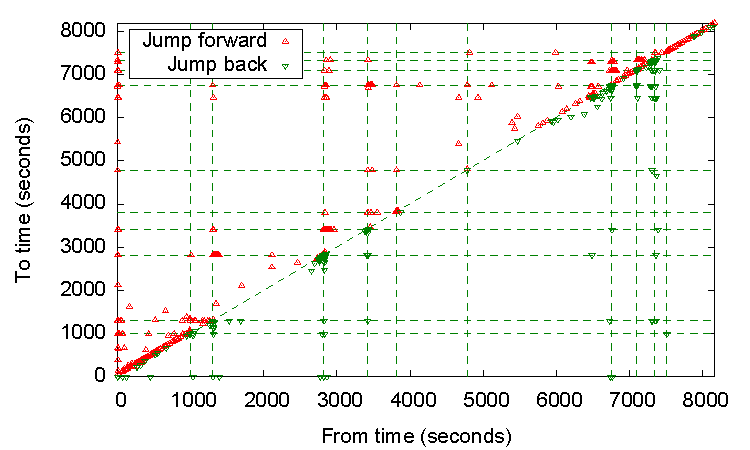
\includegraphics[width=0.5\textwidth]{./diagrams/arg-scg_jumps.pdf}
    }
    \subfloat[][Eurovision (cropped at 4000 seconds for clarity)] {
        \label{fig:eurovision_jumps}
        \includegraphics[width=0.5\textwidth]{./diagrams/eurovision_jumps.pdf}
    }

    \caption{\capttext Jumps made by users within two videos}
    \label{fig:jumps}
\end{figure}

To better understand how users navigated through a bookmarked video, we analysed the behaviour in the \emph{arg-scg} and \emph{eurovision} videos, which had 10 and 24 bookmarks respectively. In Figures~\ref{fig:argscg_jumps}~\&~\ref{fig:eurovision_jumps} each point is a seek that is identified by a ``from'' time on the x-axis and a ``to'' time on the y-axis. A point $x,y$ therefore represents a user that has jumped from their current playback point $x$ to a new point, $y$. Vertical and horizontal lines in the figures denote the position of the bookmarks. The diagonal line is a current-time marker such that seeks forward are points which lie above it, while seeks backward appear below it. Therefore, no point can fall precisely on the diagonal. It is immediately obvious from the figures that many points are on horizontal lines, implying that most seeks were to the bookmarks.

The forward seek buttons appear to have been mostly used for skipping to the next event, shown on both figures as points slightly above the diagonal line between the bookmarks. This could be due to user unfamiliarity with the bookmark interface, or possibly users simply browsing the video. Backward actions were typically used around bookmarks, where users would often re-watch the bookmarked event. In some cases users may also have wished to see video immediately preceding the bookmark. An example of this is shown in Figure~\ref{fig:argscg_jumps} before the bookmark at time 2815, where users sought up to 75 seconds backwards to see more of the build up to the goal.

Clusters of points can also be seen on horizontal lines shortly after a vertical line, indicating that users jumped from bookmark to bookmark. In fact, the concentration of clusters of point just above the diagonal time reference indicates that users have a tendency to follow bookmarks in sequence, as exemplified in Figure~\ref{fig:eurovision_jumps}.

Overall, for both videos these results demonstrate that users did not simply view continuously start-to-finish, and were in fact highly influenced when presented with bookmarks.

\subsection{Seek Distance}

\begin{figure}[tbp]
    \centering

    \subfloat[][Small scale] {
        \includegraphics[width=0.5\textwidth]{./diagrams/all_jump_distance_200}
        \label{fig:seek_distance-a}
    }
    \subfloat[][Large scale] {
        \includegraphics[width=0.5\textwidth]{./diagrams/all_jump_distance}
        \label{fig:seek_distance-b}
    }

    \caption{\capttext CDF of seek distance}
    \label{fig:seek_distance}
\end{figure}

The understanding of locality is important for caching and pre-fetching algorithms. By looking at how far users sought we can determine how close a segment has to be to have a high probability of being accessed. We therefore define \emph{seek distance} as the absolute difference, in seconds, between a user's current playback point and their requested seek destination.

Figures~\ref{fig:seek_distance-a}~\&~\ref{fig:seek_distance-b} display a CDF of seek distance for backward and forward actions. A large proportion of seeks (between 50\%-70\%) are of a 15 second, 30 second, or 60 second value. These seeks represent the short seek button presses.
40\% of backward seeks were less than or equal to 15 seconds in length. This property could be exploited by keeping a small client side buffer of previously watched segments, which would satisfy many backward seeks if the user has already viewed them.
%The seeks do not occur exactly on their respective values because seeks can only be to a video keyframe, which were not always at exact second intervals.

% forwards mean 955.32
%  'Log-Normal'    'R_SQUARE ='    [0.96622]    'TEST ='    [58.528]    'MU ='[4.7599] 'SIGMA ='    [2.5265]
%  'Weibull'    'R_SQUARE ='    [0.94271]    'TEST ='    [96.206]    'l ='    [324.87] 'k ='    [0.42302]

% backwards mean 495.95
% 'Log-Normal'    'R_SQUARE ='    [0.96888]    'TEST ='    [21.927]    'MU ='    [3.6127] 'SIGMA ='    [1.7816]
% 'Weibull'    'R_SQUARE ='    [0.95186]    'TEST ='    [34.631]    'l ='    [69.156] 'k ='    [0.6563]

% forwards > 61 with mean 1968
% 'Log-Normal'    'R_SQUARE ='    [0.99259]    'TEST ='    [8.7149]    'MU ='    [6.8269] 'SIGMA ='    [1.5953]

% backwards > 61 with mean 1630
% 'Log-Normal'    'R_SQUARE ='    [0.98238]    'TEST ='    [4.5006]    'MU ='    [6.3273]  'SIGMA ='    [1.7906]

Even though small seeks are the majority, there are between 30\% and 50\% of seeks which are further than 60 seconds. These seeks consist of jumps to bookmarks or ``blind'' seeks with the seekbar. These long range seeks are log-normally distributed with a mean of 1968 seconds and 1630 seconds for forward and backward seeks respectively. They can be fitted to log-normal models with parameters $\mu = 6.8269$ and $\sigma = 1.5953$ for forward seeks, and $\mu = 6.3273$ and $\sigma = 1.7906$ for backward seeks. This similarity implies that direction (forwards or backwards) has little impact on seek distance.

%TODO add cool stat of how many of those 40\% rewinds could be satisified frmo a buffer

These behaviours exhibit a high degree of spatial locality with the majority of seeks being within 60 seconds. Regarding long-ranged seeks, the log-normally distributed models imply that some very large distance seeks do occur, but the majority of seeks are shorter. Overall the seek distances exhibit a median of 60 seconds for forward seeks and 34 seconds for backward seeks.

\subsection{Popularity}

\begin{figure}[tbp]
    % ploted with PlotPopularityRank()
    \centering
    \includegraphics[width=0.5\textwidth]{./diagrams/all_sessions_rank}
    \caption{\capttext Object and segment popularity}
    \label{fig:popularity_object_rank}
\end{figure}

We study popularity in terms of the number of viewers who watched an \emph{object} or a \emph{segment}. An object in our system is a single video whereas a segment is a section of video one second in length.

The ranking for both object and segment popularity is shown in Figure~\ref{fig:popularity_object_rank}. The \emph{eurovision}, and \emph{arg-scg} were approximately 10,000 seconds in length, causing ~10,000 segments to be ranked for each video. Recall that only 88 videos were available, so the lowest object rank is 88. Our analysis reveals that object popularity does not follow the typical power-law distribution observed within CDNs~\cite{Chesire01Measurement,Almeida01Analysis,yu2006uub} but instead is a normal distribution with parameters $\mu = 60$ and $\sigma = 32$. This can be attributed to the nature of our videos and the relatively few new objects each day.

% object pop (using rsqare)
%'Log-Normal'    'R_SQUARE ='    [0.99735]    'TEST ='    [0.015259]    'MU ='    [4.0391]    'SIGMA ='[0.55552]
%'Normal'    'R_SQUARE ='    [0.97996]    'TEST ='    [0.11636]    'MU ='    [60.129]    'SIGMA ='    [32.111]
%'Weibull'    'R_SQUARE ='    [0.99116]    'TEST ='    [0.050083]    'l ='    [70.549]    'k ='    [2.0227]

% object pop (using kst)
%'Log-Normal'    'R_SQUARE ='    [0.99708]    'TEST ='    [0.03116]    'MU ='    [4.03]    'SIGMA ='[0.55872]
% 'Normal'    'R_SQUARE ='    [0.97993]    'TEST ='    [0.077785]    'MU ='    [59.79]    'SIGMA ='    [30.131]
%'Weibull'    'R_SQUARE ='    [0.99039]    'TEST ='    [0.05571]    'l ='    [69.301]    'k ='    [2.114]


\begin{figure}[tbp]
    \centering

    %plotted with PlotViews()

    \subfloat[][Argentina vs. Serbia and Montenegro] {
        \label{fig:arg-scg_views}
        \includegraphics[width=0.5\textwidth]{./diagrams/arg-scg_views}
    }
    \subfloat[][Eurovision] {
        \label{fig:eurovision_views}
        \includegraphics[width=0.5\textwidth]{./diagrams/eurovision_views}
    }

    \caption{\capttext Number of viewers at each second of video (each vertical line represents the position of a bookmark)}
\end{figure}

% euro (using rsquare)
%'Log-Normal'    'R_SQUARE ='    [0.99254]    'TEST ='    [0.035621]    'MU ='    [2.3233]    'SIGMA =' [0.56684]
%'Poisson'    'R_SQUARE ='    [0.95483]    'TEST ='    [0.24824]    'l ='    [11.142]
%'Weibull'    'R_SQUARE ='    [0.97982]    'TEST ='    [0.095445]    'l ='    [12.782]    'k ='    [1.8621]


% euro (using kst)
%'Log-Normal'    'R_SQUARE ='    [0.98993]    'TEST ='    [0.047187]    'MU ='    [2.3188]    'SIGMA ='    [0.49565]
%'Poisson'    'R_SQUARE ='    [0.95477]    'TEST ='    [0.14129]    'l ='    [11.132]
%'Weibull'    'R_SQUARE ='    [0.97678]    'TEST ='    [0.076196]    'l ='    [12.709]    'k ='    [2.3226]

% arg-scg (using rsqare)
%'Log-Normal'    'R_SQUARE ='    [0.99463]    'TEST ='    [0.03468]    'MU ='    [2.0063]    'SIGMA ='[0.58707]
%'Poisson'    'R_SQUARE ='    [0.98022]    'TEST ='    [0.13836]    'l ='    [8.5039]
% 'Weibull'    'R_SQUARE ='    [0.98978]    'TEST ='    [0.065082]    'l ='    [9.3509]    'k ='    [1.9405]

% arg-scg (using kst)
%'Log-Normal'    'R_SQUARE ='    [0.99428]    'TEST ='    [0.043658]    'MU ='    [2.0248]    'SIGMA ='[0.54523]
%'Poisson'    'R_SQUARE ='    [0.97926]    'TEST ='    [0.099252]    'l ='    [8.2927]
%'Weibull'    'R_SQUARE ='    [0.98943]    'TEST ='    [0.059218]    'l ='    [9.3725]    'k ='    [2.1449]

% all (using rsquare)
%'Weibull'    'R_SQUARE ='    [0.98284]    'TEST ='    [0.048803]    'l ='    [2.887]    'k ='    [0.69527]
%'Log-Normal'    'R_SQUARE ='    [0.98084]    'TEST ='    [0.054389]    'MU ='    [0.55114]    'SIGMA =' [1.3233]
%'Normal'    'R_SQUARE ='    [0.95011]    'TEST ='    [0.11357]    'MU ='    [2.5469]    'SIGMA ='    [3.4551]
%'Pareto'    'R_SQUARE ='    [0.94499]    'TEST ='    [0.13353]    'k ='    [0.97715]
%'Poisson'    'R_SQUARE ='    [0.92442]    'TEST ='    [0.2116]    'l ='    [2.923]
%'Zipf'    'R_SQUARE ='    [0.92855]    'TEST ='    [0.16903]    's ='    [1.7921]


% all (using kst)
%'Log-Normal'    'R_SQUARE ='    [0.965]    'TEST ='    [0.21597]    'MU ='    [0.95]    'SIGMA ='    [1.05]
%'Pareto'    'R_SQUARE ='    [0.94402]    'TEST ='    [0.21597]    'k ='    [1]
%'Normal'    'R_SQUARE ='    [0.93512]    'TEST ='    [0.13497]    'MU ='    [2.3933]    'SIGMA ='    [2.1693]
%'Zipf'    'R_SQUARE ='    [0.92861]    'TEST ='    [0.21597]    's ='    [1.79]
%'Poisson'    'R_SQUARE ='    [0.92163]    'TEST ='    [0.16872]    'l ='    [2.8265]

% Some matlab code to work out the top X %
% a = all_views(:,2);
% [y, x] = ecdf(a);
% x ( find(y > 0.99) ); limit = ans(1)
% sum( a ( find ( a > limit ) ) ) / sum( a )

% top 1% = 12% of requests
% top 10% = 44% of requests

The popularity of one-second segments for all the videos exhibit a Weibull distribution with parameters $\lambda=2.887$ and $k=0.69527$. Log-normal distributions provide the best fits for the  \emph{arg-scg} and \emph{eurovision} results independently with parameters $\mu = 2.00, \sigma = 0.587$ and $\mu = 2.32, \sigma = 0.567$ respectively. Note that log-normal and Weibull distributions closely relate to power-law or heavy-tailed distributions~\cite{mitz,geor06}: they are skewed distributions where a small percentage of samples contributes to a sizeable weight of their distribution. We observe that a small percentage, (the 10\% most popular segments), accounted for about 44\% of all requests. Previously, Costa~\emph{et~al.}~\cite{Costa04Analyzing} found that for educational and entertainment content, the popularity of segments is roughly uniformly distributed with a slight skew towards the beginning for entertainment content. Our result, however, implies that there are segments with orders of magnitude more viewers than others.

To illustrate the order-of-magnitude differences in viewers, we present Figures~\ref{fig:arg-scg_views}~\&~\ref{fig:eurovision_views} which show the popularity of each second of video for \emph{arg-scg} and \emph{eurovision} respectively. The vertical lines signify the position of the bookmarks; note for the \emph{eurovision} video there were no bookmarks after 6000 seconds since the performances bookmarked were only in the first half. It is clear from the figures that there are peaks of popularity, highly influenced by the bookmarks. In \emph{arg-scg} (and in other sport content) we observe that most of the bookmarks are equally popular. However in the \emph{eurovision} (and other music genres), we observe there is a greater variance in the popularity of the bookmarks. This can be attributed to sports having numerous events which all users wish to watch, however in music videos there are only some artists which interest the user.

Popularity metrics are important to many CDN algorithms as they help to decide which resources to allocate to each object. We have seen that bookmarked videos provide a content format with specific segments of interest (goals, for example). This result emphasises the use of partial caching techniques~\cite{chen2003} to cache only popular segments.

\subsection{Longevity}
\label{sect:stay_popular}

\begin{figure}[tbp]
    % plotted with PlotPopularityLifetime()
    \centering
    \includegraphics[width=0.5\textwidth]{./diagrams/all_bookpop_lifetime}
    \caption{\capttext Bookmark utilisation over time, following initial usage}
    \label{fig:lifetimes}
\end{figure}

%    'Weibull'    'R_SQUARE ='    [0.99796]    'TEST ='    [0.042635]    'l ='    [3.1004]    'k ='    [0.61592]
%    'Log-Normal'    'R_SQUARE ='    [0.98626]    'TEST ='    [0.28989]    'MU ='    [0.52115]    'SIGMA ='    [1.5475]

The popularity of both videos and bookmarks in our system faded over time. We call the duration at which any such item remains utilised its \emph{longevity}. The study of a video or bookmark's longevity can aid cache replacement policies, as well as other content management decisions.

Figure~\ref{fig:lifetimes} shows the popularity of bookmarks versus the time they were first used. The figure suggests that following an initial peak and a slight resurgence, there was a rapid decrease in interest after a short period. R-Square fitting reveals that the bookmark longevity can be suitably estimated using a Weibull distribution with $\lambda=3.10$ and $k=0.615$. This suggests that the popularity exhibits long-tailed properties. We also observe that 40\% the bookmark usage occurs within 24 hours, with the remainder slowly occurring over the following weeks.

\subsection{Session Lengths}

\begin{figure}[tbp]
    \centering
    %plotted with PlotSessions()

%    \subfigure[All videos] {
%        \label{fig:view_user_session}
%        \includegraphics[width=0.5\textwidth]{./diagrams/all_user_sessions}
%    }
    \subfloat[][Eurovision] {
        \label{fig:eurovision_user_session}
        \includegraphics[width=0.5\textwidth]{./diagrams/eurovision_user_sessions}
    }
    \subfloat[][Argentina vs. Serbia and Montenegro] {
        \label{fig:arg-scg_user_sessions}
        \includegraphics[width=0.5\textwidth]{./diagrams/arg-scg_user_sessions}
    }

    \caption{\capttext CDFs of session lengths and inter-seek times}
    \label{fig:view_user_sessions}
\end{figure}

Session length is the total time a user accessed a video, regardless of the actions they may have taken whilst doing so. For example, a session may be longer than the actual length of the video if the user chose to re-watch segments, and/or pause.

Figures~\ref{fig:eurovision_user_session}~\&~\ref{fig:arg-scg_user_sessions} show the CDF of both session and inter-seek times (discussion of inter-seek times follows in the next subsection). It can be observed from the session times that most users access each video for a very short time relative to its overall length (possibly just watching the events they are interested in). In particular, note that in the \emph{arg-scg} case around 80\% of sessions lasted less than 900 seconds. Given that the video was 2.2 hours in length, 900 seconds corresponds to only 11\% of the total video. A similar result was found with \emph{eurovision}, with 80\% of sessions lasting 12\% or less of the total video duration. The average session durations was found to be only 11 minutes and 18 minutes for \emph{arg-scg} and \emph{eurovision} respectively.

%only a small minority of users(roughly 3\%) could have possibly watched the entire match. We found that a small number of users (1.17\%) accessed the video for between 3 to 8 hours.
We also found that a small minority (roughly 3\%) of session durations were longer than the length of a video. Of these durations roughly 39\% where between 3 to 8 hours. Our logs show that these users paused for a long time before deciding to resume playback.

%These outliers are possibly why we observe that session sizes are best fitted by a log-normal distribution with parameters $\mu=4.73$ and $\sigma=1.90$.

%    'Log-Normal'    'R_SQUARE ='    [0.99779]    'TEST ='    [0.1091]    'MU ='    [4.7315]    'SIGMA ='[1.9014]
%    'Normal'    'R_SQUARE ='    [0.86057]    'TEST ='    [7.3338]    'MU ='    [143.77]    'SIGMA ='    [489.46]
%    'Weibull'    'R_SQUARE ='    [0.98666]    'TEST ='    [0.65005]    'l ='    [233.17]    'k ='    [0.51125]

\subsection{Inter-seek Times}
\label{sect:interseek}

Inter-seek time is described as the duration for which a user watched a section of a video before seeking to a new location (disregarding any paused periods). This is useful for determining the segment size to use within partial caching.

From our logs, we found that on average a user performed 8.98 seek operations around a video, resulting in a mean inter-seek time of 50.4 seconds. Figures~\ref{fig:eurovision_user_session}~\&~\ref{fig:arg-scg_user_sessions} show the CDF for inter-seek times as well as session length. As the inter-seek times are generally shorter than session times, this implies that the majority of users viewed the content as a series of excerpts, usually under a minute in length.

%It can been seen that around 50\% of viewed sections of videos were
%less than 8 seconds in length, and around 80\% of users watched the
%video for less than 50 seconds before seeking again. Less than 1\%
%of all users watched more than 1000 seconds of consecutive video.


%'Log-Normal'    'R_SQUARE ='    [0.99644]    'TEST ='    [0.020535]    'MU ='    [1.2886]    'SIGMA ='    [2.318]
%'Zipf'    'R_SQUARE ='    [0.91125]    'TEST ='    [0.36561]    's ='    [1.483]
%'Pareto'    'R_SQUARE ='    [0.92868]    'TEST ='    [0.30414]    'k ='    [0.57246]
%'Weibull'    'R_SQUARE ='    [0.99353]    'TEST ='    [0.037535]    'l ='    [7.5243]    'k ='    [0.35646]


The inter-seek time in the music content was found to be on average longer. This is because the length of a bookmarked musical performance generally exceeds the length of an event within a football match. Regardless of the difference in inter-seek times, we found that they can be estimated by log-normal distributions. For instance, the inter-seek time for \emph{arg-scg} can be modelled with parameters $\mu=2.15$ and $\sigma=1.72$.

Previous studies have found that the majority of inter-seek times are very short~\cite{vilas2005user}. For educational content, inter-seek times have also been shown to be \emph{Poisson} or \emph{Pareto} distributed~\cite{Almeida01Analysis}. We however found only $^2/_3$ of our videos had inter-seek times that could be suitably modelled by a Pareto distribution, and none that could be modelled well with a Poisson distribution. Models of inter-seek times can be used by a delivery system to determine the size of video replicas and the time available to react before a user seeks elsewhere in the video.

\subsection{Sequence}
\label{sect:sequence}

% TODO split this figure into Fig 8 and Fig 9, instead of 8a & 8b
\begin{figure}[tbp]
    \centering
    %plotted with PlotSequence()

    \subfloat[][Sequence diagram for Argentina vs. Serbia and Montenegro depicted as a tree] {
        \label{fig:sequences}
        \includegraphics[width=0.5\textwidth, height=3.6cm]{./diagrams/sequence}
    }
    \subfloat[][CDF of link probabilities for all videos] {
        \label{fig:all_sequence}
        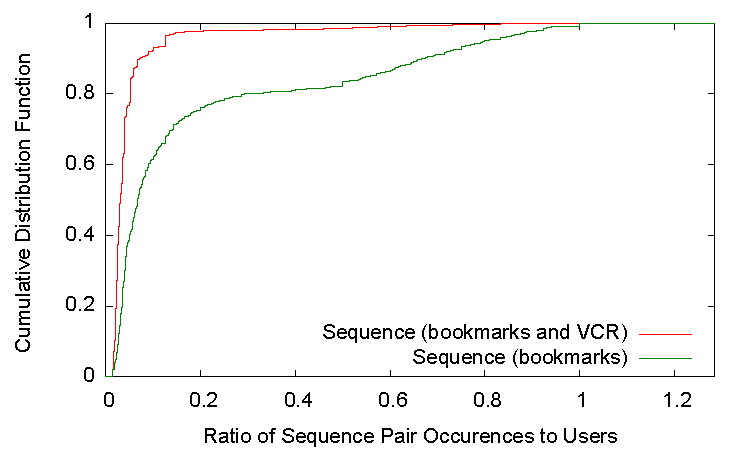
\includegraphics[width=0.5\textwidth]{./diagrams/all_sequence_normal_cdf}
    }

    \caption{\capttext Link probabilities}
\end{figure}

The traces were analysed to study the extent to which users' actions could be predicted. Since jumps to bookmarks made up a relatively large percentage of all requests, we limit this prediction to which bookmark will be visited next.
If a system could predict which bookmark would be requested next by a user, then it could pro-actively respond in order to optimise content delivery. For example, based on the next predicted bookmark, the relevant segments could be pushed out by a server with spare capacity, or pre-fetched by a client.

% 200seconds is longer than 96% of all interseek times
We call the order that bookmarks are viewed by a single user a {\em sequence} of bookmarks. Every user's sequence can be aggregated together to form a directed graph. Each node in the graph represents a bookmark with links between them representing the probability of seeking to that bookmark next. Figure~\ref{fig:sequences} shows a portion of one of these graphs depicted as a tree for clarity. The ``Start'' node represents a state before any bookmark is visited, and the ``End'' node represents the completion of a session. There is also an ``Unknown'' node which signifies when a seek to another bookmark has not been made within 200 seconds (the observed upper bound for bookmarked events' length). For clarity, links with low probabilities have also been aggregated to form a ``$N$ Others'' node, where $N$ is the number of aggregated links. It is clear from the figure that there are multiple choices to visit from each node, although there is generally one link that will have a majority probability. For example, the probability of viewing bookmark ``Goal 2-0'' immediately after ``Goal 1-0'' is 80\%.

To understand how many bookmark-to-bookmark links are predictable, Figure~\ref{fig:all_sequence} shows a CDF of probabilities for all links for all videos, as well as probabilities for just the most popular link from each bookmark. From this figure we can infer that 10\% of all links have more than a 58\% chance of being followed. %Figure~\ref{fig:all_sequence_max} shows the CDF of just the most popular link out of each node which gives a better picture of predicting what's next.
Looking at just the most popular link from each bookmark we observe that over half of the bookmarks have an outgoing link with a probability over 50\%; an encouraging result for user predictability.

%Fig.~\ref{fig:all_sequence} shows that around the top 20\% of bookmark sequence pairs were followed by more than 50\% of users. This means that there is a high chance of predicting these bookmark sequences. Note that these bookmarks also consist of the 20\% most popular bookmarks. However, the figure also shows that it is generally difficult to predict the actions of a user if all actions are considered. This is because of the wider range of interactivity options a user has when VCR functionality is also considered.

%The exact parameters are of little importance, however the type of distribution used implies the impact on the system.

%Observe that
%the {\em log-normal} distribution emerges as the best model for most
%of the observed features in our experiment, except for object
%popularity and arrival rates, which are best modelled by {\em Normal
%} and {\em Weibull} distributions respectively. This is unsurprising
%because log-normal distributions are commonly known to model various
%properties in computing systems. Weibull and, as noted earlier,
%log-normal distributions both closely relate to power-law or
%heavy-tailed distributions~\cite{geor06}.

\subsection{Hotspot Length}
\label{sect:hotspot_length}

\begin{figure}[tbp]
    \centering

    % Plotted with PlotBookmarkWaitsMerge

    \subfloat[][Argentina vs. Serbia and Montenegro] {
        \includegraphics[width=0.5\textwidth]{./diagrams/arg-scg_all_waitjumps}
        \label{fig:waitjumps-a}
    }
    \subfloat[][Eurovision] {
        \includegraphics[width=0.5\textwidth]{./diagrams/eurovision_all_waitjumps}
        \label{fig:waitjumps-b}
    }

    \caption{\capttext CDFs of wait times}
    \label{fig:waitjumps}
\end{figure}

Jumps to bookmarks comprised roughly 20\% of all requests with an additional 32\% of seeks being within 60 seconds of a bookmark. Bookmarks form the majority of requests within the content, and represent the beginning of a popular segment of video which we call a ``hotspot''. The beginning of a hotspot is generally known (the bookmark point), but the end is not. Knowing the length of the hotspot can be useful for numerous tasks such as caching and pre-fetching. We therefore define \emph{wait time} as the time elapsed between a user following a bookmark and seeking.

Figures~\ref{fig:waitjumps-a}~\&~\ref{fig:waitjumps-b} show a CDF of wait times for each bookmark in the \emph{arg-scg} and \emph{eurovision} videos. It can be seen that in the football match the wait times follow a similar distribution, with the majority of users waiting less than 40 seconds (this corresponds to the length of a run up to a goal). The \emph{eurovision} results are more varied with average wait times being much longer. This is due to the typical song in the Eurovision Song Contest being 180 seconds in length.  Finally, there is a ``Start'' bookmark listed in both figures: this is the entry point into both videos, and does not correspond to any event.

To better understand the wait times, distributions were fitted. In the general aggregated case a Weibull model fits best with parameters $\lambda=24.594$ and $k=0.7034$. For individual bookmarks log-normal and Weibull models proved best in the majority of cases.
%This result is similar to the inter-seek times in Section~\ref{sect:interseek}.
With these models the hotspots' lengths can be extrapolated by using, for example, the 95$^{th}$ percentile.

%'Log-Normal'    'R_SQUARE ='    [0.98463]    'TEST ='    [0.1127]    'MU ='    [2.6361]    'SIGMA ='    [1.388]
%'Weibull'    'R_SQUARE ='    [0.99545]    'TEST ='    [0.033063]    'l ='    [24.594]    'k ='    [0.7034]
%'Zipf'    'R_SQUARE ='    [0.93259]    'TEST ='    [0.34879]    's ='    [1.018]


\subsection{User Behaviour Models}

\begin{table}[tbp]
    \centering{\tiny
    \begin{tabular}{|c|c|c|}
      \hline
      Metric & Distribution & R-square \\
      \hline
      Object Popularity  & Normal ( $\mu=60.129$ , $\sigma=32.111$ )     & 0.97996 \\

      Segment Popularity & Log-normal ( $\mu=0.551$ , $\sigma=1.32$ )   & 0.98084 \\
                         & Weibull    ( $\lambda=2.887$ , $k=0.69527$ ) & 0.98284 \\

      Session Length     & Log-normal ( $\mu=4.73$, $\sigma=1.90$ )     & 0.99779  \\
                         & Weibull    ( $\lambda=233.17$, $k=0.51125$ ) & 0.98666 \\

      Inter-seek times   & Log-normal ( $\mu=1.2886$, $\sigma=2.318$ )  & 0.99644 \\
                         & Weibull    ( $\lambda=7.5243$, $k=0.35646$ ) & 0.99353 \\

      Seek Distance (forward)      & Log-normal ( $\mu = 7.2668$, $\sigma = 1.2194$ )  & 0.99567 \\                     Seek Distance (backward)     & Log-normal ( $\mu = 7.195$, $\sigma = 1.3132$ )   & 0.99083 \\

      Hotspot Length    & Log-normal ( $\mu=2.6361$, $\sigma=1.388$ )  & 0.98463 \\
                         & Weibull    ( $\lambda=24.594$ , $k=0.7034$ ) & 0.99545 \\

      Bookmark Longevity & Weibull    ( $\lambda=3.1004$ , $k=0.61592$ ) & 0.99796 \\
    \hline
    \end{tabular}
    }
    \caption{\capttext A summary of metrics with their corresponding distributions}
    \label{tab:models}
\end{table}

Model fitting is important for understanding the different properties of the system, and aids in simulation creation and algorithmic design. Various models have been discussed for the different parameters of the system. In all cases many models (\emph{e.g.}, normal, log-normal, exponential, Weibull, Pareto, Poisson, Zipf) were fitted to the data with varying success. Generally, more than one distribution fitted well. This subsection will summarise the analytical models found for each parameter.

Table~\ref{tab:models}, gives an overview of the best matching models for each metric discussed previously, with their corresponding \emph{R-square} values. Of particular importance are the types of distribution which can have a significant impact on the system. For example, the Weibull and log-normal models are both long-tailed, and systems may have to anticipate the skewed distribution to cope effectively.

The models shown so far are from aggregated results across all the videos. However, it may be interesting to model the different metrics of each particular video. Table~\ref{tab:models_all} lists the number of videos for each metric which can be modelled with an \emph{R-square} value greater than 95\%. The ``max models'' column represents the number of datasets that are of sufficient size to have models fitted. For example, there are 695 bookmarks, yet only 203 had enough data to be fitted with a hotspot length.

\begin{table}[tbp]
    \centering{\tiny

    \begin{tabular}{|c|c|c|c|c|c|c|c|c|}
      \hline
      Metric & Max Models & Log-normal & Weibull & Pareto & Normal & Exponential & Zipf & No fit\\
      \hline

      Segment Popularity & 84 (from 88 videos) & 61  & 65  & 12 & 58 & 42 & 13 & 17\\
      Session Length     & 81 (from 88 videos) & 75  & 72  & 0  & 5  & 31 & 4  & 0\\
      Inter-seek times   & 87 (from 88 videos) & 83  & 83  & 54 & 1  &  3 & 55 & 3\\
      Hotspot Length    & 203 (from 695 bookmarks) & 165 & 135 & 91 & 5  & 48 & 53 & 22 \\

      \hline
    \end{tabular}

    }\caption{\capttext Metrics for individual videos and their corresponding distributions}
    \label{tab:models_all}
\end{table}

\subsection{Summary}

%In this section we have shown:
%    When presented with bookmarks users are highly influences by them
%    This causes the popularity of seconds to be heavy-tailed
%    Session times are very short compared to media
%    A sequence of bookmarks can be predicted
%
%    Can we make sure bookmarks help the system as much as possible?
%    Can we predict which bookmark is next?

Our results have shown that the interactivity options available to users highly influence their behaviour. In particular, it was found that the novel interactive feature of \emph{bookmarking} played a pivotal role, leading to access patterns quite dissimilar from previous related studies that looked at VCR-like interactivity alone.
The combination of our content type and the addition of bookmarks led to users accessing content in relatively short segments sparsely distributed throughout the length of the videos. Segment popularity is skewed with the most popular segments clearly around the bookmarks, forming hotspots. From both a user and a CDN's perspective, this can be viewed as advantageous; users can reach interesting content more quickly through the bookmarks, and the increased locality of interest means CDNs can respond more effectively by, for example, prioritising hotspot replication.

Content placement is an important and difficult problem for CDNs. The CDN has to decide where within the network to replicate or cache content. Typically the content is placed near to the users, and replicated as a whole. However, as we have seen, not all segments within a piece of content are equal and a CDN can leverage this information to replicate certain segments more than others. This is especially useful when popularity nearly always concentrates around bookmarks, allowing the relevant segments to be replicated throughout the network before user demand increases.

A CDN could be designed to handle high levels of user interactivity, with relatively short session and inter-seek times. Our results have shown that hotspots following bookmarks were orders of magnitude shorter than the video containing them. Furthermore, it encourages the use of an agile delivery mechanism that allows distribution of small sparsely distributed segments quickly and efficiently.

We have also shown that users view the bookmarks in a similar order, giving them a degree of predictability. This could allow a CDN to exploit pre-fetching techniques to improve the user's experience. For example, if the CDN could predict the next segment the user will watch, then this could be pre-fetched into the user's playback buffer and when the user seeks to that segment there will be no delay caused by seek latency and buffering.

The use of bookmarks depends on them being well positioned and of interest to the user. We noted in the first experiment that 40\% of bookmarks had at least one user seek before the bookmark, with 30.7\% of these seeks occurring within 5 seconds of jumping to the bookmark. This perhaps represents users who were almost immediately dissatisfied with the bookmark's location. We noted this happened consistently for roughly 6\% of the total bookmarks. Upon further inspection, it appeared the bookmarks were inadvertently misplaced. This led to users performing additional seeks to find the correct location, thus placing extra load on the servers.

In Section 5~\ref{sect:new_techiques}, we explore and study the implications of two techniques designed to exploit some of the properties suggested from our analysis. %The first addresses the dynamic re-positioning of bookmarks in response to user behaviour. The second concerns predictive pre-fetching of popular segments to enhance the efficiency of delivery of highly interactive content.

\section{Techniques for Interactivity Support}
\label{sect:new_techiques}

% simple dynamic bookmark placement and interactivity-aware content pre-fetching and replication

During our second video trial, we took the opportunity to go beyond characterising user behaviour, by testing autonomic content management techniques in a live system. In this section we discuss and analyse a simple dynamic bookmark placement technique, as well as an interactivity-aware content pre-fetching method based on the prediction of which bookmark would be viewed next.

\subsection{Moving Bookmarks}
\label{sect:moving_bookmark}

During our video trials, bookmarks were appropriately positioned by administrators before the video was published. It was previously noted that a small percentage of bookmarks were unintentionally misplaced. There are many reasons why a bookmark could be misplaced, such as human error, or a lack of insight into user requirements. For example: a bookmark could be placed before a penalty kick, but many users may first wish to see the foul that led to the penalty. As such, it could be beneficial if the system could autonomically detect poorly placed bookmarks and correct them based on feedback derived from the user's actions.

%For example a football goal bookmark would be placed at the position the scoring team gained possession of the ball just before the goal. This allowed the user to view the run up to the goal, as well as the goal itself.


\begin{figure}[tbp]
    \centering

    %TODO Come up with some clever way to pre-compile this
    \input{./diagrams/scenarios.tex}

    \caption{Different scenarios that may induce bookmark movement}
    \label{fig:movingbookmark}
\end{figure}

To develop a reactive algorithm that moves bookmarks dependent on user behaviour, different possible scenarios should first be explained. Figure~\ref{fig:movingbookmark} shows three different sequences of actions a user would follow shortly after seeking to a bookmark.

\emph{Scenario A} shows the user briefly viewing the bookmark, then seeking to a time earlier than it. While this could indicate that the bookmarked event was short and that the user wanted to view it again, it could equally imply that the bookmark was placed later than it should have been.

\emph{Scenario B} is similar to \emph{Scenario A} but differs in that the user does not seek back to a point before the bookmark; this means the user is simply replaying footage, thus implying the bookmark is correctly placed for that individual.

\emph{Scenario C} represents a situation in which the user's motives are difficult to determine. Since they watch briefly then seek forward, several possibilities exist: the bookmarked event may have ended, the bookmark may have been placed prematurely, or the user is simply seeking forward towards the next event.

A further possibility, not shown in the figure, is for a user to seek far away from a bookmark in either direction. Since it is unlikely their destination would be related to the bookmark, such an action would not indicate the bookmark was incorrectly placed.

\emph{Scenario A} and \emph{Scenario C} are therefore the only scenarios where the user's actions could indicate the bookmark is misplaced. All other actions should reinforce the position of the bookmark to reduce future movements once it is correctly placed. Additionally since we are less sure of the user's intentions in \emph{Scenario C} we should only make minor changes to the bookmark's placement to limit the impact of false-positives.

Algorithm~\ref{alg:bookmark} has been developed to identify these situations and act appropriately with regard to moving a bookmark. An exponential moving average (EMA) is used to recalculate the bookmark's position with a smoothing constant $\alpha$. The value used for $\alpha$ is dependent on the identified scenario, allowing us to place greater confidence in the seeking-backward \emph{Scenario A} than the seeking-forward \emph{Scenario C}. For our testing scenario we used a maximum wait times of 20 and 60 seconds for backward and forward seeks respectively. These maximum values were chosen because they exceeded approximately 80\% of all wait times.

%Note that 20s is used in the algorithm because 81.7\% of backward seeks were carried out in that interval, and 87.49\% of forward seeks within 60s}

%Scenario C can work in a similar way to A, but since since forward jumps are less accurate, the parameters need to change. Alpha should be lower to reduce the movement, a higher period to wait for the jump and a limit on the distance between the bookmark and the jump location.
%Another idea is to move the bookmark by the inverse of the distance jumped. So if the user jumps a long distance then perhaps the bookmark wasn't incorrectly placed, and instead they are jumping to a new location. However if the jump is small then perhaps they are looking for for the event, and thus the bookmark should be move more.
%More data is needed on early bookmarks to find out the sequence of events.

%\[ B_{t+1} = \left\{
%    \begin{array}{ll}
%         1          & \mbox{if $S_{t} < B_{t}$}\\
%         0          & \mbox{if $B_{t} \le S_{t} \le (B_{t} + w)$} \\
%         1          & \mbox{if $S_{t} > B_{t}$}
%    \end{array}
%\right. \]

\renewcommand{\algorithmiccomment}[1]{// #1}
\begin{algorithm}
{\small
\begin{algorithmic}[0]
    \STATE\COMMENT{$B_{t}$ is the location of the bookmark at time $t$}
    \STATE\COMMENT{$S_{t}$ is the location the user sought at time $t$}
    \STATE\COMMENT{$w$ is the time the user waited before seeking to $S_{t}$}
    \IF {$S_{t} < B_{t}$}
        \STATE\COMMENT{\emph{The user seeks backwards before the bookmark}}
        \IF {$w <= 20$ \textbf{and} $S_{t} > (B_{t} - 60)$}
            \STATE\COMMENT{\emph{The seek occurred within 20 seconds of viewing the bookmark and landed within 60 seconds of the bookmark}}
            \STATE $\alpha = 0.1$
            \STATE $B_{t+1} = \alpha S_{t} + (1-\alpha) B_{t}$
        \ENDIF

    \ELSIF {$S_{t} > (B_{t} + w)$}
        \STATE\COMMENT{\emph{The user seeks forward}}
        \IF {$w <= 60$ \textbf{and} $S_{t} < (B_{t} - 120)$}
            \STATE\COMMENT{\emph{The seek occurred within 60 seconds of viewing the bookmark and landed within 120 seconds of the bookmark}}
            \STATE $\alpha = 0.05$
            \STATE $B_{t+1} = \alpha S_{t} + (1-\alpha) B_{t}$
        \ENDIF
    \ENDIF
\end{algorithmic}
}
\caption{Bookmark moving algorithm}
\label{alg:bookmark}
\end{algorithm}



\begin{figure}[tbp]
    \centering

    \subfloat[][Position over time] {
        \label{fig:man-mil-time}
        \includegraphics[width=0.5\textwidth]{./diagrams/mufc-mila_Goal_3-2_time}
    }
    \subfloat[][Position over requests for bookmarks] {
        \label{fig:man-mil-requests}
        \includegraphics[width=0.5\textwidth]{./diagrams/mufc-mila_Goal_3-2_request}
    }

    \caption{\capttext Manchester United vs Milan single bookmark position}
    \label{fig:man-mil}
\end{figure}

To test this algorithm, several of the bookmarks in our second video trial (not our initial World Cup experiment) were deliberately misplaced by different amounts both before and after the apparently correct point. Over time the bookmarks were moved by our algorithm. For example, Figures~\ref{fig:man-mil-time}~\&~\ref{fig:man-mil-requests} show the position of a single bookmark as it was moved autonomically by the system with respect to time and received requests. In both cases the system responds and the bookmark quickly moves to a new position, and then gradually converges until it becomes stable.

\begin{figure}[tbp]
    \centering

    \subfloat[][CDF of percentage reduction in viewing duration] {
        \label{fig:duration_saved_cdf}
        \includegraphics[width=0.5\textwidth]{./diagrams/moved_savedovertime_cdf}
    }
    \subfloat[][Percentage reduction in viewing duration versus received requests] {
        \label{fig:duration_saved_requests}
        \includegraphics[width=0.5\textwidth]{./diagrams/moved_binned_savedovertime}
    }

    \caption{\capttext Reduction in viewing duration due to the algorithm}

\end{figure}

%\todo{ Make reduction calc clearer }

It is subjective to decide if a bookmark has moved to its correct location, so we instead look at how much traffic has been saved by moving the bookmark to a new location. If, for example, a bookmark was moved forward 10 seconds closer to the desired location, and a user views for 90 seconds, then by moving the bookmark we have potentially stopped 10 seconds of video being transferred which might have normally been skipped over. A reduction of $10/(90+10)=10\%$ is therefore made. Of course, this is only true if the user does not seek backward to watch the skipped 10 seconds, in which case we save nothing, and in fact incur an extra seek. Figure~\ref{fig:duration_saved_cdf} displays a CDF of the potential reduction in viewing duration per bookmark request from the use of the algorithm. We can see that 16\% of the requests made no saving: these are accounted for by early requests before the bookmarks were moved, and requests where the user seeks between the original and current bookmark location. %The remaining 84\% of request reduced the play

Figure~\ref{fig:duration_saved_requests} illustrates how rapidly these reductions are made (and whether or not they are sustainable) through a plot of the fractional potential saving versus the number of requests received across all the moved bookmarks. For the first 20\% of requests the reductions are low yet they improve, and then stabilise at a reduction of between 30-40\% per request. The 95\% confidence interval is quite wide in most cases (averaging around $\pm$10 seconds) although this variance is mostly due to differences in playback length and not the 16\% of requests with no saving.

With minimal processing this simple algorithm has been able to reposition the bookmarks to more appropriate locations based on observed user behaviour, resulting in consistent reductions.

%\begin{figure}[tbp]
%    \centering
%    \includegraphics[width=0.5\textwidth]{./diagrams/sequence.png}
%
%    \caption{\capttext Graph of the order bookmarks are clicked. Note: This is a work in progress, and doesn't display well so I'll send links around to larger pngs.}
%%    \label{fig:mil-man}
%\end{figure}

%   Before  After   Distance            Best
%mufc-mila_Goal 1-2 3185    3168    17  Late            *interesting, because bookmark was well placed (but got moved)
%mufc-mila_Goal 3-2 7431    7409    22  Late        7417.808
%liv-che_Goal 1-0   2286.185    2187    99.185  Late
%ita-fra_Penalty 1-0    3915.718    3904    11.718  Late
%mil-man_Goal 3-0   8433.083    8415    18.083  Late
%mil-man_Goal 2-0   4505    4473    32  Late
%mil-man_Goal 1-0   3260    3277    -17 Early       3299.81

%notes
%Rates of seeks over time
%Find the end of bookmark
%change the sequence graphs (to show direction, correct weights), and possible add another "didn't jump" state
%what time do they jump out?

% How many times was a segment re-watched, and how soon between watching? Indicates how useful local buffering old content would help

%Figures~\ref{fig:man-mil} show the position of a single bookmark in the Manchester United vs Milan over time. This bookmark was purposely placed too late by 15 seconds, causing frustrated users to rewind. Figures~\ref{fig:mil-man} shows the placement of a Milan vs Manchester United bookmark which was placed 30 seconds too early.


\subsection{Predictive Pre-fetching}

Due to the increased interactivity of users and their departure from the start-to-finish model, it is no longer wise to simply pre-fetch ahead of the playback point. However, as noted in Section~\ref{sect:sequence} it is still possible to predict which bookmarked segment of video a user will view next, allowing the client to intelligently pre-fetch content, benefitting both client and server. For the client, pre-fetching removes seek latency when seeking to a pre-fetched segment, both in terms of the network seek latency incurred and also the time taken to buffer enough video for playback (as well as helping to avoid buffer underruns under poor network conditions). Similarly, on the server side pre-fetching can help reduce the peak server load, by increasing the load at quieter times with pre-fetching requests, thus making the overall load more uniform.
%Figure~\ref{fig:server_load_a} gives an example of server load at different times. The shaded areas show the server going over some limit, perhaps the server's bandwidth capacity. If pre-fetching is used this load could happen earlier whist staying below the server's limit as shown in Figure~\ref{fig:server_load_b}.

However, pre-fetching does come with a cost, as resources are wasted if a segment is downloaded and never used. Deciding which segments to pre-fetch is therefore a difficult task. We used different pre-fetching strategies, each using different information to decide which segment to fetch next. For simplicity, and because interest always formed around bookmarks, each strategy will only pre-fetch segments immediately following a bookmark (bookmark hotspots). %Hotspots always focused around bookmarks therefore these were a good choice to prefetch. However the length of these hotspots were not always know, so as you will see later, arbitrary values were used for the length of the pre-fetched segment.
{\parindent0ex
The different pre-fetching strategies tested are explained as follows:

    \textbf{Before Start} pre-fetches all the bookmark hotspots before the user begins any playback. This demonstrates how well pre-fetching everything in advance will perform.

    \textbf{Best} uses knowledge of future events to pre-fetch the bookmark hotspot that the user is actually going to view next. This is impossible to implement in practice, so this technique is for reference only. %Similar to Belady's minimum.

    \textbf{Predictive} uses knowledge observed from other users as to which bookmark is likely to be requested next, and thus starts to pre-fetch the bookmark hotspots in descending order of probability of being visited. The greater the number of users interacting with the system, the more accurate the predictive knowledge becomes.

    \textbf{Sequence} simply pre-fetches bookmark hotspots in the order in which they appear within the video.

    \textbf{Sequence After} again simply pre-fetches bookmark hotspots in the order in which they appear within the video. This technique will however only pre-fetch segments that are after the current playback point.

    \textbf{Random} will pre-fetch the bookmark hotspots in a random order.

    \textbf{Popularity} pre-fetches the bookmark hotspots in order of their overall popularity.

}

Simulations were run using real \emph{eurovision} traces obtained from our system to test these different strategies. \emph{Eurovision} was chosen due to its popularity and  representative nature. As soon as the client starts playback of a video a separate thread begins to pre-fetch segments (at playback rate) which the scheme anticipates the client will need. Connections between the clients and server were highly provisioned and never congested. In all experiments the amount pre-fetched for each bookmark was determined by varying the percentile of that particular bookmark's length model, as described in Section~\ref{sect:hotspot_length}.


\begin{figure}[tbp]
    \centering

    \subfloat[][Fraction of requests with zero seek latency] {
        \label{fig:eurovision_instaseek}
        \includegraphics[width=0.5\textwidth]{./diagrams/1194827971-eurovision_tab-instaseek}
    }
    \subfloat[][Pre-fetched usage ratio] {
        \label{fig:eurovision_usage}
        \includegraphics[width=0.5\textwidth]{./diagrams/1194827971-eurovision_tab-usage}
    }
    % TODO: crop this plot

    \subfloat[][Pre-fetch cache hit/miss ratio] {
        \label{fig:eurovision_ratio}
        \includegraphics[width=0.5\textwidth]{./diagrams/1194827971-eurovision_tab-ratio}
    }

    \caption{\capttext Various metrics for different pre-fetch schemes versus bookmark length}

\end{figure}

To begin with the number of requests with zero seek latency were counted. These occur when the user has already pre-fetched at least 1 second of video from a requested seek point. Figure~\ref{fig:eurovision_instaseek} displays the fraction of all seeks which could instantly be served from data pre-fetched. As expected, the \emph{Before Start} and \emph{Best} schemes outperformed all others. The \emph{Predictive} and \emph{Sequence After} schemes both performed equally catching at most 23\% of seeks, and the \emph{Popularity}, \emph{Sequence} and \emph{Random} schemes also performed equally albeit roughly 5\% lower than the \emph{Predictive} and \emph{Sequence After} schemes.
It is interesting to note that using the popularity of the bookmark is not as effective as using the somewhat na\"{\i}ve \emph{Sequence} scheme. This is because while the \emph{Popularity} scheme is pre-fetching the most popular bookmarks (which could be towards the end of the video), the \emph{Sequence} scheme is fetching closer bookmarks which will be used sooner.
As the pre-fetch size becomes larger most schemes are able to offer more zero latency seeks due to aiding seeks that occur shortly after the bookmark (\emph{e.g.}, seeking 15 seconds forward). However the improvements begin to diminish around 60\% as excess data is pre-fetched and thus time would be better spent fetching a different bookmark.

Each scheme may pre-fetch different amounts of data. For example, the \emph{Best} scheme will keep trying to pre-fetch the bookmark hotspot that the user will view next, but if there is no following bookmark the scheme stops pre-fetching. Figure~\ref{fig:eurovision_usage} displays the amount pre-fetched data that was actually used for playback. The \emph{Best} scheme performs at least twice as well as any other listed, with the \emph{Before Start} performing worse since it has pre-fetched far more data than actually gets used. From the remaining schemes, \emph{Predictive} is consistently the best, achieving between 31\% and 39\% usage.

Finally, we observe the overall byte hit/miss ratio in Figure~\ref{fig:eurovision_ratio}. This is how many bytes were successfully served by pre-fetched data versus the total number of bytes requested. Again, the different schemes performed similarly, with \emph{Predictive}, \emph{Sequence After}, and \emph{Popularity} performing equally. However, none of the schemes, including \emph{Before Start} achieved a satisfactory hit-ratio. At best, the realistic schemes achieved less than 20\%. This may be because the bookmark hotspots do not sufficiently cover the area requested by the users. Future work could therefore incorporate strategies that pre-fetch more than just hotspots following a bookmark.

From these results it is clear the \emph{Predictive} and \emph{Sequence After} schemes perform best, with the \emph{Predictive} scheme slightly outperforming \emph{Sequence After} by having a higher pre-fetched utilisation. One aspect that has not been investigated is how quickly reliable knowledge needed for the \emph{Predictive} scheme can be obtained through other users' interactions. As such, a hybrid approach could be taken, beginning by using the simple yet effective \emph{Sequence After} scheme, switching to the \emph{Predictive} scheme once sufficient statistics have been acquired.

The \emph{Best} scheme outperformed all others which suggests room for improvement in the other pre-fetching algorithms. The results presented are, however, perhaps the worst case since each client is working independently. If the clients collaborated, a shared pre-fetching network cache could result, thus increasing the hit/miss ratios while decreasing the load on the CDN.

\section{Conclusions and Future Work}
\label{sect:conclusion}

%Summary
%    Bookmarks highly influence behaviour,
%    this breaks existing CDN,
%    however CDNs can exploit this,
%    for example sequence prediction,
%    and bookmark moving?
%    lots of models!

We have presented a study and characterisation of user behaviour for our interactive Video-on-Demand system. We note that by adding simple bookmarks to points of interest within the media, the access patterns are greatly influenced. This behaviour led to high levels of seeking which created relatively-short and sparsely-distributed segments with orders of magnitude more popularity than others.

Various distributions were fitted to the different metrics considered, providing a greater understanding of how users interact with such systems. Beyond the insight gained, the models constitute a valuable toolbox for driving future simulations which require highly interactive workloads.

Many existing delivery mechanisms are not designed for high levels of interactive behaviour and are instead optimised for classic start-to-finish streaming. CDNs must therefore adapt to efficiently handle these kinds of access patterns. They could, for example, take advantage of the long-tailed distributions of segments by replicating those that generate the most demand. For instance, we observed that 10\% of segments accounted for 44\% of all requests.

The departure from classic start-to-finish playback encourages the design of agile delivery mechanisms that allow quick seeking, and allow certain more popular segments to be more highly distributed. We have seen that adding bookmarks will highly influence the order in which users view the content, making the sequence of actions somewhat predictable. This can then be exploited by allowing users to pre-fetch content that they are predicted to need shortly, thus reducing any delays they are likely to experience. However, we noted that bookmarks could be harmful if incorrectly placed by causing unnecessary seeks. This could be remedied for both client and server by simply moving the bookmark autonomically based on observed user behaviour.

%Future work -
%    We have only looked at music and sports, does this apply to others? How does very typical start-to-finish media with bookmarks act when users are present with bookmarks?
%
%    Automatic bookmark generation
%    Discussion of "next bookmark" (could be useful if the bookmark was generated automatically)
%
%    Beyond bookmarks, ie prefetching other segments
%    How quickly can we collect/calculate predictive data.
%    Do the clients pre-fetch, or does the server do the work (or just offer recommendations)?
%    Different forms of pre-fetching, in parallel, etc
%
%    Design of  agile delivery mechanism that allows distribution of small sparsely distributed segments quickly and efficiently.

So far we have only considered bookmarks within music and sport videos, but bookmarks are equally applicable in many other genres. For example, bookmarks are commonly found in the form of chapters in movies released on DVD. It is not clear if the same high levels of interactivity would be observed, or if the classic start-to-finish model would still be prevalent.

For a system to be fully autonomic the bookmarks should perhaps be created automatically. This could occur after the system has detected a large number of requests for a specific area of a video. A bookmark could then be provisionally placed and its position refined by a bookmark-moving algorithm, such as the one found in Section~\ref{sect:moving_bookmark}.

During our experiment users were unhappy that we ``spoilt the experience'' of watching the sporting events covered somewhat. This was because the user could quickly determine the final outcome from the bookmark names. The suggestion was made that we avoid labelling the bookmarks and instead simply describe them as points of interest. This could equally work if the bookmarks were autonomically created since a system would be unable to name them itself. Note, unnamed bookmarks would only be useful if they are typically accessed sequentially, and not based on their name alone.

It was clear from Figure~\ref{fig:eurovision_ratio} that pre-fetching only segments shortly following bookmarks only covered 30\% of viewed segments. Thus pre-fetching schemes should consider more segments. This of course would make it harder to decide which segments to pre-fetch next. The probability of making a wrong decision could be reduced if the pre-fetching was done in different ways, such as pre-fetching more than one choice simultaneously.

% todo: consider emulating users most like yourself, rather than the majority

The predictive pre-fetching algorithms used knowledge inferred from the observations of other users. For example, if the majority of all users visited two bookmarks in the same order, it is likely the next user will do the same. How this knowledge is collected, how this knowledge is disseminated, and how quickly this knowledge becomes useful is left open for future study. We did not discuss how this knowledge would be used, and indeed both the client and server could exploit it differently, each with respective pros and cons. For example, if the client has spare capacity, it could start to pre-fetch based on both its own previous behaviour and that of the majority of other users. The server could also decide to pre-replicate, or to push out segments predicted to be required when it has spare capacity.

High levels of interactivity are becoming more common, whilst users are both relying on and expecting Video-on-Demand services to provide more advanced interactive functionality. Our study suggests that CDN mechanisms must improve to handle more diverse applications, content and users. To achieve this, the development of new algorithms must be driven by models derived from realistic characterised workloads. The development of such strategies is reliant on gaining a deep understanding of the relevant workload parameters. The analysis and models presented in this paper aim to aid in this endeavour.

\bibliographystyle{abbrv}
\bibliography{worldcup}

\end{document}
